\section{From Interpretations to Nested Trees}
\label{sec:ramseyan}

\subsection{From Interpretation to Monoids}

\AP In this section, we will use standard construction from automata theory,
and especially the equivalence between $\MSO$-formulas on trees and bottom-up
deterministic tree-automata. We refer to the book on Tree Automata Techniques
and Applications for a comprehensive overview of this topic \cite{TATA08}. It
follows from standard arguments that to a formula $\varphi(x,y)$ over binary
trees labelled using letters in $\Sigma$ one can associate a monoid $M$ and a
morphism $\mu \colon \Sigma^* \to M$ such that for any tree $T$ and any pair of
leaves $x,y$ in $T$, whether $T \models \varphi(x,y)$ is entirely determined by
the values of $\mu(T[z \colon x])$, $\mu(T[z \colon y])$ and $\mu(T[\treeRoot
\colon z])$ where $z = \lca(x,y)$ is the \kl{ least common ancestor} of $x$ and
$y$.
As a consequence,
one can collect in a subset $P \subseteq M^3$ all the triples $(a,b,c)$ such
that this triple corresponds to a satisfying assignment of the formula
$\varphi(x,y)$.
This is illustrated in \cref{interpretation-to-monoid:fig}. 

\AP In order to simplify notations and better distinguish between the labels of
the nodes (in a finite alphabet $\Sigma$) and their corresponding elements in
the monoid $M$, we will label the \emph{edges} of the trees by the elements of
$M$, having a special treatment for the root of the tree. Given two nodes $x
\treelt[T] y$ in a tree $T$, we will write $\tlbl{T}{x}{y}$ for the product of
the edge labels on the path from $x$ to $y$ in $T$.  Furthermore, we assume for
the rest of the section that the monoid $M$ and the morphism $\mu$ are fixed,
together with the accepting part $P \subseteq M^3$. As a consequence, when we
refer to trees in this subsection, they have nodes labelled by $\Sigma$ and
edges labelled by $M$. Given such a tree $T$, we define $\treeSem{T}$ as the
graph obtained by considering leaves of $T$ as vertices, and placing an edge
between two leaves $x$ and $y$ if and only if $(\tlbl{T}{z}{x}, \tlbl{T}{z}{y},
\tlbl{T}{\treeRoot}{z}) \in P$ where $z = \lca(x,y)$.

\begin{figure}
    \centering
    \begin{tikzpicture}[
        leaf/.style={
            color=Prune
        },
        lca/.style={
            color=A1
        },
        edge/.style={
            color=A2
        },
        root/.style={
            color=Prune
        },
        gedge/.style={
            color=A4
        },
        ]
        \node[root] (root) at (0,1) {$\treeRoot$};
        \node[leaf] (x) at (-1,-1) {$x$};
        \node[leaf] (y) at (1,-1) {$y$};
        \node[lca] (lca) at (0,0) {$\lca(x,y)$};
        \coordinate (tl) at ($(x.south west)+(-0.2,0)$);
        \coordinate (tr) at ($(y.south east)+(0.2,0) $);
        \coordinate (t)  at ($(root.north)+(0, 1)$);
        \draw[edge,->] (root) to node[midway, left]        {$a$}  (lca);
        \draw[edge,->] (lca)  to node[midway, above  left] {$b$} (x);
        \draw[edge,->] (lca)  to node[midway, above right] {$c$} (y);
        \draw (tl) -- (tr) -- (t) -- cycle;

        \node (maps-to) at (3,0) {$\mapsto$};

        \begin{scope}[xshift=4cm]
            \node[leaf] (nx) at (0,0) {$x$};
            \node[leaf] (ny) at (5,0) {$y$};
            \draw[gedge] (nx) to node[midway, above] {$(a,b,c) \in P$?} (ny);
        \end{scope}
    \end{tikzpicture}
    \caption{The interpretation of a tree using a monoid and an accepting part.}
    \label{interpretation-to-monoid:fig}
\end{figure}

The main idea of using monoids to encode the truth value of $\varphi(x,y)$ is
that one can then use a suitable notion of tree embeddings makes the
interpretation from trees to graphs \emph{monotone}.

\begin{definition}
    \label{composition-ordering:def}
    Let $T_1$ and $T_2$ be two trees. 
    A map $h \colon T_1 \to T_2$ is an \intro{compositional tree embedding}
    if it is a \kl{tree embedding} and
    for all pairs of nodes $x \treelt[T_1] y$ in $T_1$, 
    we have $\tlbl{T_1}{x}{y} = \tlbl{T_2}{h(x)}{h(y)}$.
\end{definition}

\begin{lemma}
    \label{composition-ordering:lem}
    Let $T_1$ and $T_2$ be two trees such that
    $h \colon T_1 \to T_2$ is a \kl{compositional tree embedding}.
    Then, $h \colon \treeSem{T_1} \to \treeSem{T_2}$
    is a \kl{labelled graph embedding}.
\end{lemma}
\begin{proof}
\end{proof}

\AP As a consequence, it is sufficient to understand when the \kl{composition
ordering} on trees is well-quasi-ordered to understand when the \kl{labelled
graph embedding} is well-quasi-ordered. Historically, this was (although not
explicitly) the approach taken by \cite{DRT10}. Unfortunately, the composition
ordering on trees is more often than not way more strict than the \kl{induced
subgraph} ordering. It was already observed that the composition ordering on
trees is \kl{well-quasi-ordered} if and only if \emph{for every} $Q \subseteq
M^3$, the class of graphs obtained from trees by considering only the triples
in $Q$ is \kl{labelled-well-quasi-ordered} \cite{LOPEZ24}. To understand what
happens for a precise choice of $Q$, we need to have a finer understanding of
the way trees can be decomposed.




\begin{figure}
    \centering
    \todo[inline]{Draw the composition ordering on trees}
    \caption{The composition ordering on trees}
    \label{composition-ordering:fig}
\end{figure}

\subsection{Forward Ramseyan Splits}

\def\t{\aTree} \AP The crucial combinatorial ingredient to understand how to
decompose further the trees will come from an adaptation of the classical Simon
Factorisation Theorem for semigroups \cite{SIMO90}, adapted to trees by
Colcombet \cite{COLC07}. A \intro{split of height $N$} of a tree $\t$ is a
mapping $\spt$ from the nodes of $T$ to $\set{1, \dots, N}$. Given a split
$\spt$ and two nodes $x \treelt[\t] y$, we define $\spt(x \colon y)$ to be the
minimal value of $\spt(z)$ for $x \treelt[\t] z \treelt[\t] y$, and $\infty$
otherwise. Two elements $x \treelt[\t] y$ such that $\spt(x) = \spt(y) = k$ are
\intro{$k$-neighbours} if $\spt(x \colon y) \geq k$.

\AP A split $\spt$ is \intro{forward Ramseyan} if for every $k \in \set{1,
\dots, N}$ and every $x, y, x', y'$ in the same class of \kl{$k$-neighbourhood}
with $x \treelt[\t] y$ and $x' \treelt[\t] y'$, we have:
\begin{equation}
    \label{fake-idempotent:eq} 
    \tlbl{\t}{x}{y} = \tlbl{\t}{x}{y} \cdot \tlbl{\t}{x'}{y'} \quad .
\end{equation} 

\AP
In particular, $\tlbl{\t}{x}{y}$ is an \kl{idempotent}, since $\tlbl{\t}{x}{y}
\cdot \tlbl{\t}{x}{y} = \tlbl{\t}{x}{y}$, but $\tlbl{\t}{x}{y}$ and
$\tlbl{\t}{x'}{y'}$ may be different \kl{idempotents}. 

\AP Let us illustrate how one can use \kl{forward Ramseyan splits} to compute
efficiently the value of $\tlbl{\t}{x}{y}$ for any pair of nodes $x \treelt[\t]
y$. We are going to paraphrase the actual content of \cite[Lemma 3]{COLC07},
using the drawing of \cref{fast-computation:fig} to explain the idea. We claim
that to compute the value of $\tlbl{\t}{x}{y}$, one can restrict the
computation to \emph{few} specific segments of the path from $x$ to $y$ with a
\emph{strictly larger} value of $\spt$. The reason is that whenever $x$ and $y$
are separated by many nodes $z$ such that $\spt(z) = \spt(x:y)$, one can
essentially ignore all but the first and last such nodes to speed up
computation. This of course can be applied recursively leading to a fast (and
first-order definable, provided the split $\spt$ is known) algorithm to compute
the value of $\tlbl{\t}{x}{y}$.

\begin{figure}
    \centering
    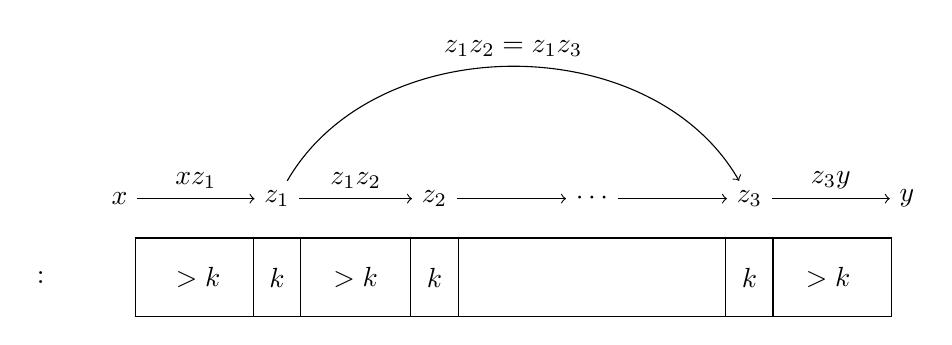
\begin{tikzpicture}
        \node (s) at (-1,-1) {$\spt \colon $};
        \node (x) at (0,0) {$x$};
        \node (z1) at (2,0) {$z_1$};
        \node (z2) at (4,0) {$z_2$};
        \node (z3) at (6,0) {$\cdots$};
        \node (z4) at (8,0) {$z_3$};
        \node (y) at (10,0) {$y$};

        \node[below of=z1] {$k$};
        \node[below of=z2] {$k$};
        \node[below of=z4] {$k$};
        \node (xz1) at (1,-1) {$> k$};
        \node (z1z2) at (3,-1) {$> k$};
        \node (z4y) at (9,-1) {$> k$};

        \draw (0.2,-0.5) rectangle (9.8,-1.5);
        \draw (1.7,-0.5) -- (1.7, -1.5);
        \draw (2.3,-0.5) -- (2.3, -1.5);

        \draw (3.7,-0.5) -- (3.7, -1.5);
        \draw (4.3,-0.5) -- (4.3, -1.5);

        \draw (7.7,-0.5) -- (7.7, -1.5);
        \draw (8.3,-0.5) -- (8.3, -1.5);


        \draw[->] (x) -- 
        node[midway, above] {$\tlbl{\t}{x}{z_1}$}
        (z1);
        \draw[->] (z1) --
        node[midway, above] {$\tlbl{\t}{z_1}{z_2}$}
        (z2);
        \draw[->] (z2) -- (z3);
        \draw[->] (z3) -- (z4);
        \draw[->] (z4) -- 
        node[midway, above] {$\tlbl{\t}{z_3}{y}$}
        (y);
        \draw[->] (z1) to[bend left=60] 
        node[midway, above] {$\tlbl{\t}{z_1}{z_2} = \tlbl{\t}{z_1}{z_3}$}
        (z4);

    \end{tikzpicture}
    \caption{Fast computation of the value $\tlbl{\t}{x}{y}$
        provided a forward Ramseyan split.}
    \label{fast-computation:fig}
\end{figure}

\AP The main theorem of \cite{COLC07} is that for every finite monoid $M$,
there exists a finite depth $N$ such that for every tree $T$ labelled using
$M$, there exists a forward Ramseyan split of height $N$ for $T$. We can
therefore assume that our trees are always equipped with a forward Ramseyan
split of height $N$.

\AP One can define a notion of embedding between two trees equipped with their
respective \kl{forward Ramseyan splits}. Given two trees $\t_1$ and $\t_2$ with
their respective splits $\spt_1$ and $\spt_2$, a map $h \colon \t_1 \to \t_2$
is a \intro{gap embedding} if it is a \kl{tree embedding} and for all
\kl{$k$-neighbouring} nodes $x \treelt[\t_1] y$ in $\t_1$, $h(x) \treelt[\t_2]
h(y)$ are \kl{$k$-neighbouring} nodes in $\t_2$. Trees equipped with
\kl{forward Ramseyan splits} form a \kl{well-quasi-ordered} set with respect to
the \kl{gap embedding} relation \cite{DERSHOWITZ200380}.

\AP Let us introduce a notion of dependency between nodes that will allow us to
explain how the \kl{gap embedding} relation preserves \emph{some} of the monoid
products in the trees. A node $x$ is \intro{independent at level $k$} from a
node $y$, written $x \bot_k y$ if $x$ is \kl{independent at level $k+1$} and
$\spt(x:y) \geq k+1$ or if there exist three nodes $z_1, z_2, z_3$ such that
$x \treelt[\t] z_1 \treelt[\t] z_2 \treeleq[\t] z_3 \treelt[\t] y$ such that
$\spt(z_1) = \spt(z_2) = \spt(z_3) = k$, $x \bot_{k+1} z_1$, $z_1 \bot_{k+1}
z_2$, and $z_3 \bot_{k+1} y$. If $k = N+1$, then $x \bot_{N+1} y$ if $x$ is the
immediate ancestor of $y$ in the tree.

\begin{lemma}
    Let $h \colon (T, \spt) \to (T', \spt')$ be a \kl{gap embedding} between two
    trees equipped with \kl{forward Ramseyan splits}. Then, for all $x \bot_k y$
    in $T$, we have $\tlbl{T}{x}{y} = \tlbl{T'}{h(x)}{h(y)}$.
\end{lemma}
\begin{proof}
    By immediate induction on $\spt(x:y)$.
\end{proof}

